\documentclass[a4paper, 12pt]{article}

\usepackage{graphicx}
\usepackage{xcolor}
\usepackage{mdframed}
\usepackage { amsmath , amssymb , amsthm }
\usepackage[T2A]{fontenc}
\usepackage[utf8]{inputenc}
\usepackage[english,russian]{babel}

\graphicspath{{img/}}
\DeclareGraphicsExtensions{.pdf,.png,.jpg}


\title{Домашнее задание по теме "Двойные и тройные интегралы"}
\author{Осипенко Д. 595гр.}
\date{\today}

\begin{document}
\sffamily
\maketitle
\section*{6}
\[
	\iint_{D}{e^{ x+\sin y} \cos y dx dy} \quad \{(x,y)|0 \leq x \leq \pi ,0 \leq y \leq \pi/2 \}
\]
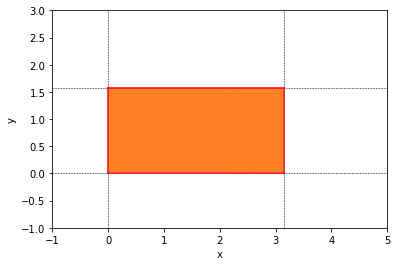
\includegraphics{img/index.jpg}\\
\[
		\int_{0}^{\pi/2}dy \int_{0}^{\pi}(e^{ x+\sin y} \cos y)dx =\int_{0}^{\pi/2}(e^{ \pi+\sin y} - e^{\sin y})d(\sin y) =
\]
\[
	(e^{ \pi+\sin y} - e^{\sin y})\big|_{0}^{\pi/2}= \underline{(e^{ \pi+1} - e) - (e^{ \pi} - 1) }
\]
\section*{7}
\[
	\iint_{D}{(x^2+y^2) dx dy} \quad y=x,x=0,y=1,y=2
\]
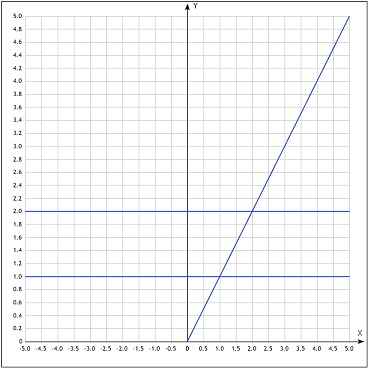
\includegraphics{img/1.png}
\[
	\int_1^2dy\int_0^2(x^2+y^2)dx = \int_1^2(\frac{8}{3}+2y^2)dy = \frac{8}{3}+\frac{16}{3} - \frac{8}{3}-\frac{2}{3}=\underline{\frac{14}{3}}
\]
\section*{31}
\[
	\iint_{D}{ \frac{dx dy}{x^2+y^2+1}} \quad y=\sqrt{1-x^2} ,y = 0
\]
\[
	\int_0^{\pi}d\theta\int_0^1\frac{rdr}{r^2(\cos^2\theta+\sin^2\theta)+1} = \frac{r}{r^2 +1}\big|_0^1 \cdot \theta\big|_0^\pi = \underline{\frac{\pi}{2}}
\]
\section*{33}
\[
	\iint_{D}{ \frac{\sin \sqrt {x^2+y^2}}{\sqrt{x^2+y^2}} dx dy} \quad x^2+y^2=\pi^2/9,x^2+y^2=\pi^2 
\]
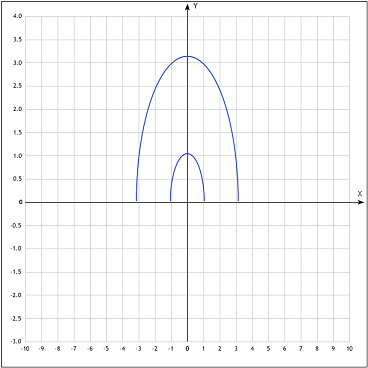
\includegraphics{img/2.png}
\[
	\int_0^\pi d\theta\int_{\frac{\pi}{9}}^\pi\frac{\sin \sqrt {r^2}}{\sqrt{r^2}}rdr = \frac{r\sin r}{r}\big|_{\frac{\pi}{9}}^\pi\cdot\theta\big|_0^\pi = \frac{\pi\pi\sin \pi}{\pi}-\frac{\pi\frac{\pi}{9}\sin \frac{\pi}{9}}{\frac{\pi}{9}} = 
\]
\[
	\underline{-\pi\sin \frac{\pi}{9}}
\]












\end{document}